            
            
            \begin{figure}
            \begin{subfigure}
                \centering
                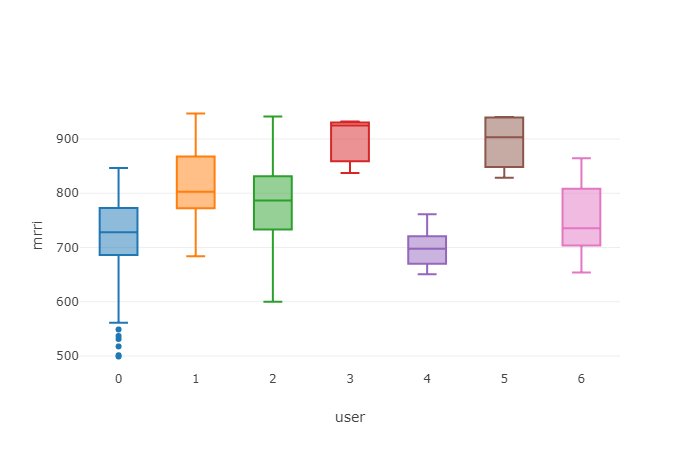
\includegraphics[width=0.85\textwidth]{sessions/sess_box_mrri_all.png}
                \caption{Distribuição da média de intervalos por sessão para cada indivíduo para atividades excluindo exercício, sono e movimento}
                \label{sess_box_mrri_all}
            \end{subfigure} 
            \begin{subfigure}
                \centering
                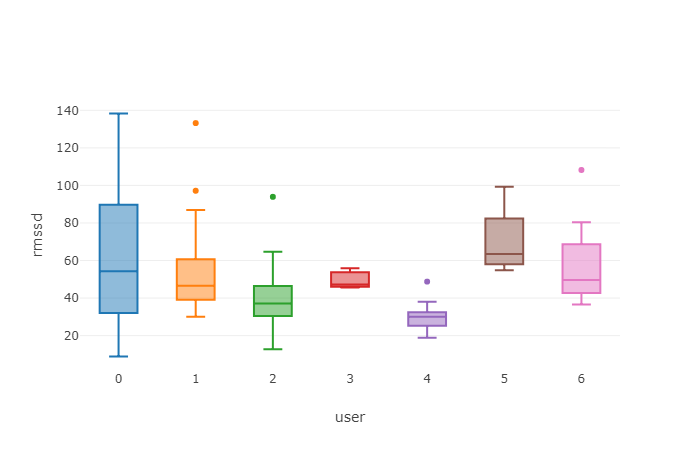
\includegraphics[width=0.85\textwidth]{sessions/sess_box_rmssd_all.png}
                \caption{Distribuição da média RMS da diferença entre  intervalos consecutivos por sessão para cada indivíduo para atividades excluindo exercício, sono e movimento}
                \label{sess_box_rmssd_all}
            \end{subfigure} 
            \end{figure}

            
            
            \begin{figure}%
                \centering
                \subfigure[][]{%
                    \label{fig:ex3-a}%
                    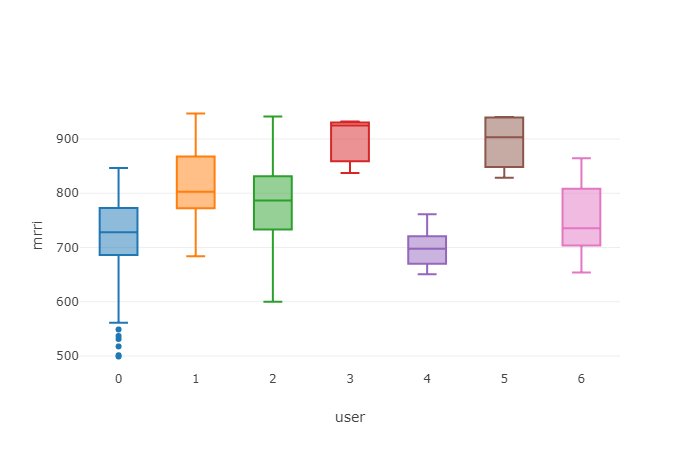
\includegraphics[width=0.5\textwidth]{sessions/sess_box_mrri_all.png}}%
                \subfigure[][]{%
                    \label{fig:ex3-b}%
                    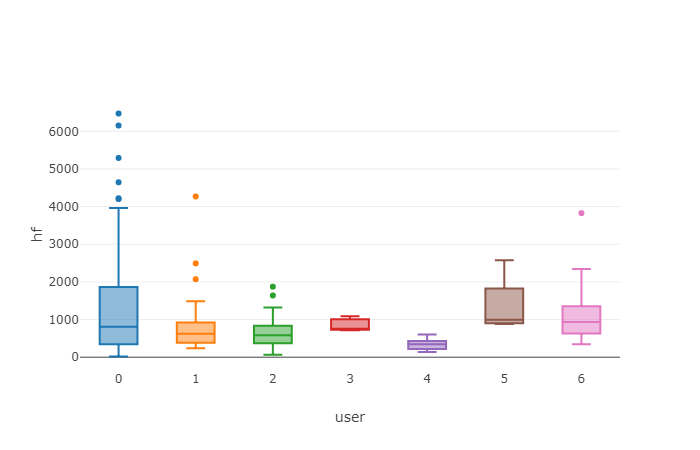
\includegraphics[width=0.5\textwidth]{sessions/sess_box_hf_all.png}} \\
                \subfigure[][]{%
                \label{fig:ex3-c}%
                    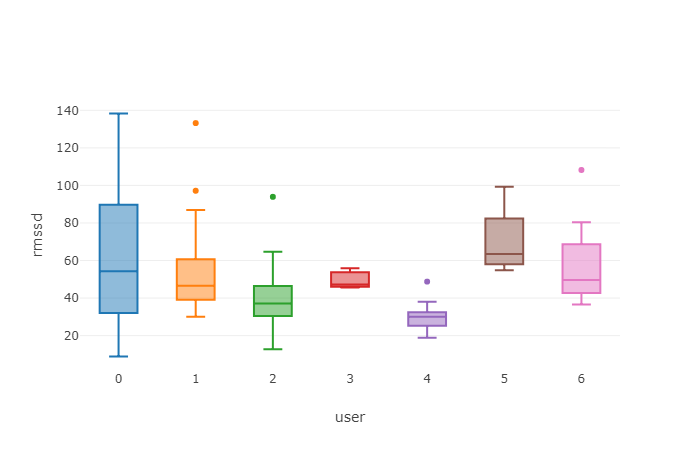
\includegraphics[width=0.5\textwidth]{sessions/sess_box_rmssd_all.png}}%
                \subfigure[][]{%
                \label{fig:ex3-d}%
                    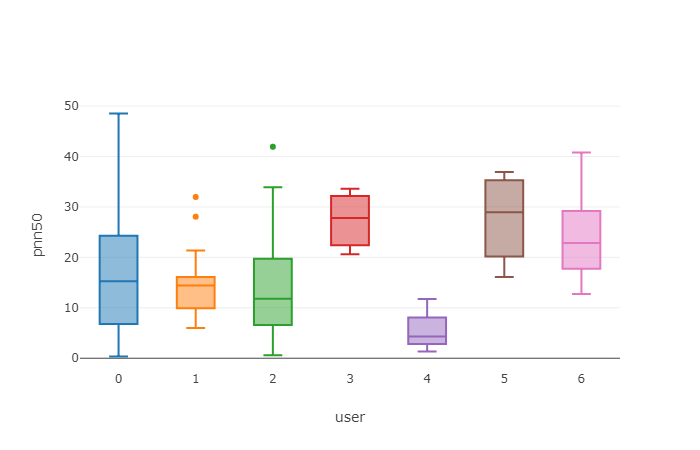
\includegraphics[width=0.5\textwidth]{sessions/sess_box_pnn50_all.png}}%
                    \caption[A set of four subfigures.]{A set of four subfigures:
                    \subref{fig:ex3-a} describes the first subfigure;
                    \subref{fig:ex3-b} describes the second subfigure;
                    \subref{fig:ex3-c} describes the third subfigure; and,
                    \subref{fig:ex3-d} describes the last subfigure.}%
                \label{sess-boxplot-all}%
            \end{figure}
            
             
            \begin{figure}%
                \centering
                \subfigure[][]{%
                    \label{fig:ex3-a}%
                    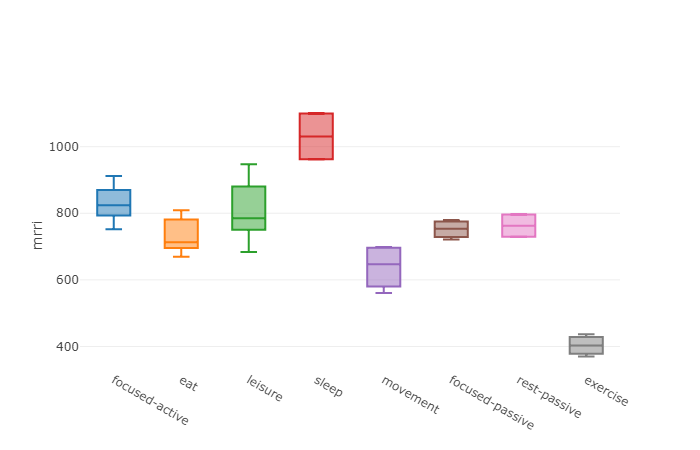
\includegraphics[width=0.5\textwidth]{sessions/sess_box_mrri_ronald.png}}%
                \subfigure[][]{%
                    \label{fig:ex3-b}%
                    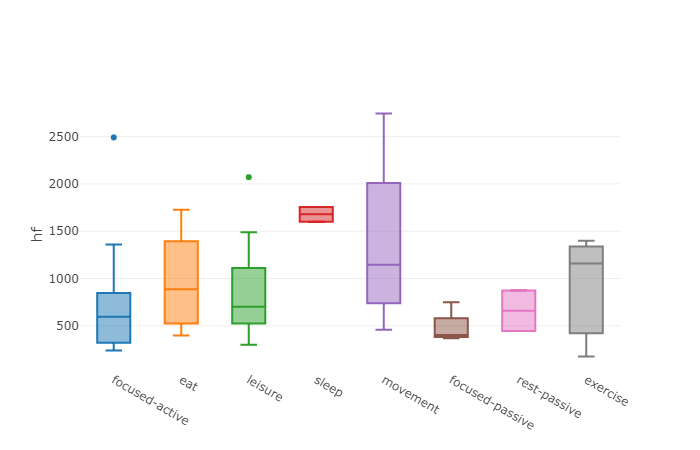
\includegraphics[width=0.5\textwidth]{sessions/sess_box_hf_ronald.png}} \\
                \subfigure[][]{%
                \label{fig:ex3-c}%
                    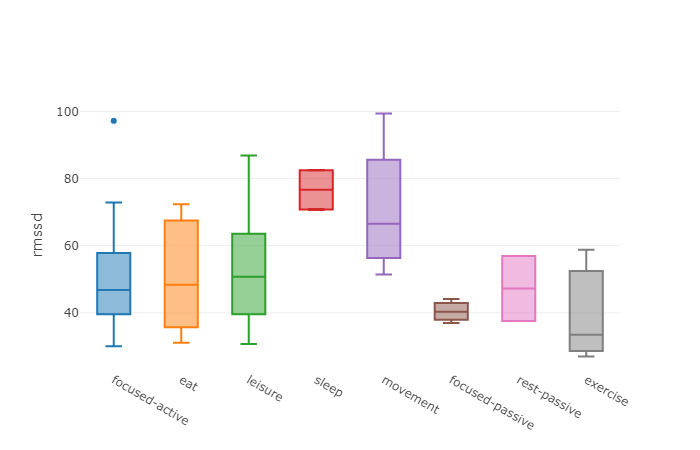
\includegraphics[width=0.5\textwidth]{sessions/sess_box_rmssd_ronald.png}}%
                \subfigure[][]{%
                \label{fig:ex3-d}%
                    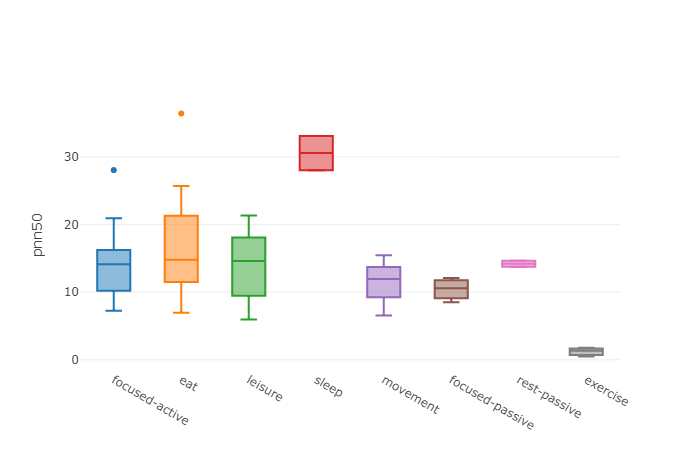
\includegraphics[width=0.5\textwidth]{sessions/sess_box_pnn50_ronald.png}}%
                    \caption[A set of four subfigures.]{A set of four subfigures:
                    \subref{fig:ex3-a} describes the first subfigure;
                    \subref{fig:ex3-b} describes the second subfigure;
                    \subref{fig:ex3-c} describes the third subfigure; and,
                    \subref{fig:ex3-d} describes the last subfigure.}%
                \label{sess-boxplot-ronald}%
            \end{figure}
